\begin{englishtitle}
\title{Hysteresis loop in neural networks with simplices of different orders}
% First author
\author{Kirill Ryabov}
\institute{Higher School of Economics, Nizhniy Novgorod, Russia\\
  \email{ksriabov@edu.hse.ru}
   }
% etc

\maketitle

\begin{abstract}
The study focuses on the behavior of neural networks with various types of simplex connections, specifically the search for hysteresis effects. One of the most widely used models for this purpose is the Kuramoto equation, which allows us to analyze the behavior of large numbers of interconnected oscillators. A variant considered in this study is a network of oscillators in which each node is connected to all other nodes, also known as a network of globally coupled oscillators. The change in a key parameter has been examined numerically, and when a clear jump is observed in the resulting graph, hysteresis can be identified. When the system is integrated backwards in time, the resulting pattern resembles a classic loop

\keywords{hysteresis effect, Kuramoto equation, neural networks }
\end{abstract}
\end{englishtitle}


\iffalse
\documentclass[12pt]{llncs}
\usepackage[T2A]{fontenc}
\usepackage[utf8]{inputenc}
\usepackage[english,russian]{babel}
\usepackage[russian]{nla}

%\usepackage[english,russian]{nla}

% \graphicspath{{pics/}} %Set the subfolder with figures (png, pdf).

%\usepackage{showframe}
\begin{document}
%\selectlanguage{russian}
\fi

\title{Явление гистерезиса в нейронных сетях с симплексами различных порядков }
% Первый автор
\author{К.~С.~Рябов
} % обязательное поле
\institute{Высшая школа экономики, Нижний Новгород, Россия\\
  \email{ksriabov@edu.hse.ru}
   }
% Другие авторы...

\maketitle

\begin{abstract}
Исследование посвящено поведению нейронных сетей с симплекс связями различных порядков, а именно отысканию эфекта гистерезиса. Одна из самых популярных моделей для этого -- уравнение Курамото. При ее помощи можно рассмотреть поведение большого числа связанных между собой осцилляторов.Рассмотрен вариант, где связь среди нейронных узлов --   все со всеми, который еще называют сетью глобальных осцилляторов.Численно расмотрено изменение параметра порядка и при наблюдении явного скачка на этом графике можно детектировать гистерезис. При интегрировании системы в обратном времени картина соответсвует классической петле. 
  

\keywords{явление гистерезиса, уравнение Курамото, нейронные сети}
\end{abstract}

\section{Основные результаты} % не обязательное поле
Запишем уравнение, которое задает динамику изменения узлов в нейронном слое с течением времени :
\begin{equation}\dot{\theta_i}= \omega_i+\frac{K1}{N}\sum^{N}_{j=1} \sin(\theta_j-\theta_i)+\frac{K2}{N^2} \sum^{N}_{j=1} \sum^{N}_{k=1}  \sin (2\theta_j-\theta_k-\theta_i).\end{equation}
В данной формуле $\theta_i$ -- фаза и $\omega_i$ -- частота i-го осциллятора, $k$ -- сила связи между элементами.
Будет использовать симплексы до 2го порядка включительно, так вклад вклад симлексов более высоких связей не вносит значительный вклад.

 Симплексами будем называть n-мерное обобщение треугольника. Таким образом, симплексом первого порядка будет называть отрезок, а симплексом второго порядка-треугольник.

 Для отыскания петли гистерезиса необходимо рассмотреть явление фазовой синхронизации. Её критерием является параметр порядка.
Приведем его формулу: 
\begin{equation} r  =\frac{1}{N} \sum^{N}_{i=1} e^{i \theta_i}, \end{equation} если мы получили, $r=0$, значит   нет фазовой синхронизации, а случай $r=1$ соответсвует случаю фазовой синхронизации осцилляторов. Но примимать значения он может любые из отрезка $[0;1]$.

Для проведения численных исследований необходимо задать начальные распределения в формуле (1). Будем использовать иследующие фазы :$\omega$ будут распределены по Коши с параметрами (0, 0.5), а частоты $\theta$, в свою очередь, будут распределены равномерно в пределах от $0$ до $2\pi$.

Зафиксируем количество осцилляторов на значении $N=25$, то есть количество узлов 625.
Для того, чтобы найти условие возникновения синхронного режима нашей модели проведём численное интегрирование системы методом Рунге-Кутты 4-го порядка: шаг по времени $dt=0.01$ на времени $T=1000$.
 \begin{figure}
\center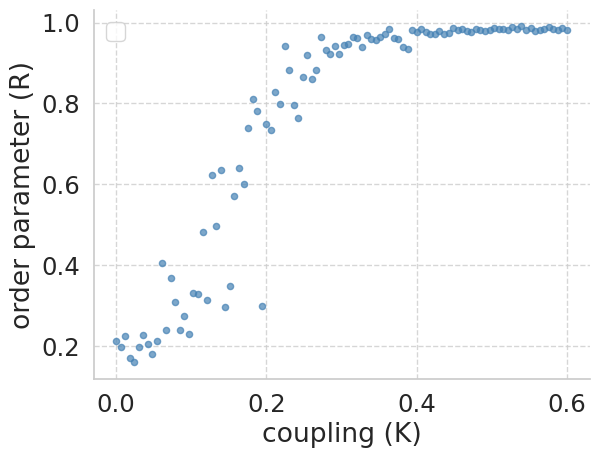
\includegraphics[height=6cm]{aRyabovris3.png}
 \caption{Изменение параметра порядка при N=25 от параметра $K $ в  связях с симплексами первого порядка.}
\end{figure}

Как мы видим, осцилляторы можно явным образом разделить на 2 кластера: те, где синхронизация произошла, и где ее нет. Переход происходит достаточно плавно, но есть некоторый разброс точек. Не произошло резкого перехода подозрительного на явление гистерезиса. Поэтому рассмотрим симлексы второго порядка.
При интегрировании при тех же параметрах получим следующую кртину.
 \begin{figure}
\center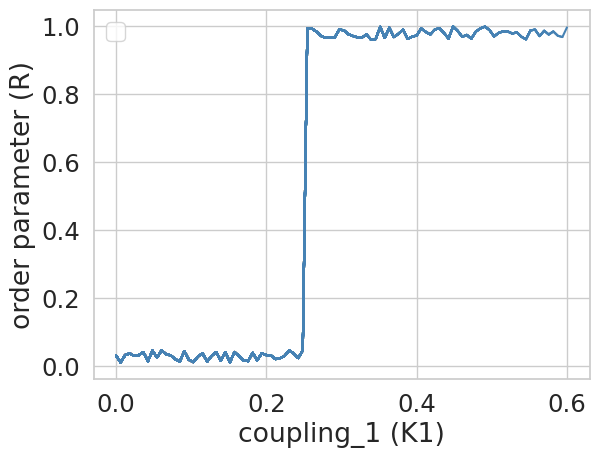
\includegraphics[height=6cm]{aRyabovris2.png}
 \caption{Изменение параметра порядка при N=25 от параметра $K_1$ в  связях с симплексами второго порядка.}
\end{figure}

Видим, что в отличии от симплексом первого порядка, тут переход происходит не так плавно (скачком). Резко возникает бассейн глобально синхронизованных осцилляторов. 

При итегрировании в обратном времени мы видим явную петлю гистерезиса.
\begin{figure}
\center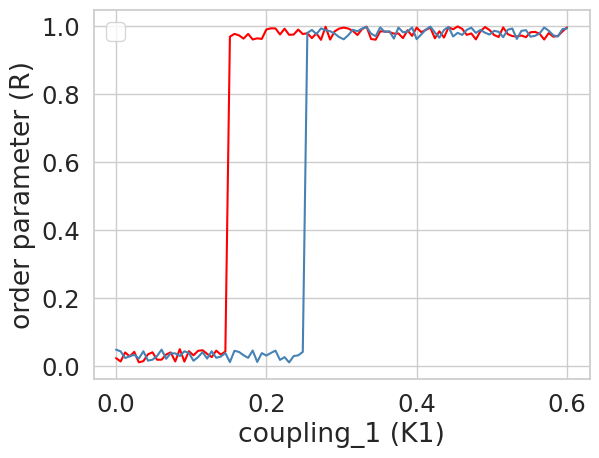
\includegraphics[height=6cm]{aRyabovris1.png}
 \caption{Явление гистерезиса в сетях с симплексами второго порядка.}
\end{figure}

Кривую полученную при интегрировании изобразим синим цветом, при интегрировании в обратном цвете обозначим красным. 
Мы видим, что значение параметра $K_1$, при котором происходит скачковый переход, отличается. На красной прямой он находится левее относительно синей. 


% Список литературы.
\begin{thebibliography}{99}
\bibitem{1}
% Format for Journal Reference
 Winfree A.T.  { Biological rhythms and the behavior of populations of coupled oscillators}.   J. Theor. Biol. 1967. Vol. 16  Pp.~15--42.
% Format for books
\bibitem{2}
Kuramoto Y. Chemical Oscillations. Waves and Turbulence. Berlin: Springer-Verlag, 1984.
% Format for Russian Journal Reference
\bibitem{3} Kuramoto Y. {   Self-entrainment of a population of coupled non-linear oscillators In: Araki H}. International Symposium on Mathematical Problems in Theoretical Physics, Lecture Notes in Physics. Berlin: Springer-Verlag, 1975. Vol. 39, Рp.~420--422.
% etc
\end{thebibliography}





%\end{document}

%%% Local Variables:
%%% mode: latex
%%% TeX-master: t
%%% End:
